% figure: 自控-死区双积分结构图.png
% 用途：自控 08-2-2 描述函数判据与自振例题 —— 死区非线性 + 双积分对象的闭环结构；
%       与同一节的相平面闭轨图（自控-死区双积分操场形闭轨.png）配套。
% 构建：..\build.ps1 -File .\block-deadzone.tex
\documentclass[border=10pt]{standalone}
\usepackage{fontspec}
\setmainfont{Cambria}
\usepackage{unicode-math}
\setmathfont{Cambria Math}
\usepackage{tikz}
\usetikzlibrary{positioning, arrows.meta, calc}
\usepackage{ctex}

\definecolor{figink}{HTML}{1E2228}
\definecolor{figsub}{HTML}{606874}
\definecolor{figfill}{HTML}{E8EFF8}

\begin{document}
\begin{tikzpicture}[
  x=1cm, y=1cm,
  line width=0.95pt, line cap=round, line join=round,
  >=Stealth,
  blk/.style = {draw=figink, line width=0.95pt, fill=figfill,
                minimum height=0.9cm, inner sep=4pt,
                anchor=center, font=\small, align=center},
  sum/.style = {draw=figink, line width=0.95pt, circle, inner sep=0pt,
                minimum size=0.42cm, anchor=center},
  sig/.style = {font=\small, color=figink},
  lbl/.style = {font=\small, inner sep=1.5pt},
  sub/.style = {font=\footnotesize, color=figsub}
]

\node[sum] (s1) at (0,0) {};
\node[blk, minimum width=2.4cm] (nz) at (2.6,0) {死区非线性};
\node[blk, minimum width=2.2cm] (g)  at (6.0,0) {$G(s)=\dfrac{1}{s^2}$};

\draw[->] (-2.4,0) -- node[sig, above] {$r$} (s1.west);
\draw[->] (s1.east) -- node[sig, above] {$e$} (nz.west);
\draw[->] (nz.east) -- node[sig, above] {$u$} (g.west);
\draw[->] (g.east) -- (9.0,0);
\node[sig] at (9.0,0.30) {$c$};
\fill (8.3,0) circle (1.6pt);
\draw[->] (8.3,0) -- (8.3,-2.0) -- (0,-2.0) -- (s1.south);

\node[lbl] at (-0.36,0.32) {$+$};
\node[lbl] at (-0.46,-0.32) {$-$};
\node[sub] at (2.6,-1.05) {$|e|\le2:\ u=0$，其外斜率 $1$};
\node[sub] at (4.2,-1.72) {负反馈};

\end{tikzpicture}
\end{document}
